\documentclass{article}
\usepackage[a4paper,margin=1in,footskip=0.25in]{geometry}
\usepackage{tikz}
\usetikzlibrary{spy,shapes,shadows,calc,pgfplots.groupplots}
\usepackage{amsmath}
\usepackage{amsfonts}
\usepackage{amssymb}
\usepackage{stmaryrd}
\usepackage{graphicx}
\usepackage{epstopdf}
\usepackage{algorithmic}
\usepackage{enumitem}
\usepackage{booktabs}
\usepackage{pgfplotstable}
\usepackage{colortbl}

\pgfplotstableset{% global config
    every head row/.style={before row=\bottomrule,after row=\hline},
    every last row/.style={after row=\toprule},
}

\providecommand{\abs}[1]{\left\lvert#1\right\rvert}
\providecommand{\norm}[1]{\left\lVert#1\right\rVert}

\newcommand{\drawSquare}{\begin{tikzpicture}
\node[ ] at (0,0) {\textcolor{blue}{\nullfont\pgfuseplotmark{square}}};
\end{tikzpicture} }
\newcommand{\drawCircle}{
\begin{tikzpicture}
\node[ ] at (0,0) {\textcolor{red}{\nullfont\pgfuseplotmark{o}}};
\end{tikzpicture} }
\newcommand{\drawTriangle}{\begin{tikzpicture}
\node[ ] at (0,0) {\textcolor{green!70!black}{\nullfont\pgfuseplotmark{triangle}}};
\end{tikzpicture}
}
\begin{document}

\begin{figure}[h]
\begin{center}
\begin{tikzpicture}[scale = 1.0]
\begin{scope}[ ]
\begin{tiny}
\begin{axis}[
    height = 4.15cm,
    width = 5.45cm,
    name=displ,
    ymode=log,
    xmode=log,
    ymax = 7e-1,
    axis y line*=left,
    xlabel= { $\Delta t = h$},
    x label style={at={(axis description cs:0.75,+0.31)},anchor=east},
    y tick label style={ xshift=2.85em,yshift=0.6em },
    ytick = {1e-3,1e-6},
    legend style = { column sep = 10pt, legend columns = 1, legend to name = grouplegendnoGCC,},
    %title = {  $\norm{ \cdot }_{L^{\infty}(0,T;L^2(\Omega))}$ vs.  $\norm{ \cdot }_{L^{\infty}(0,T;L^2(B_t))}$  },
    title = { $ u$ in $ \Omega$ (solid) vs $ B_t $ (dashed) }, 
    title style={at={(0.5,1.0735)},anchor=north},
    legend style={at={(0.5,-0.0)},anchor=north},
    ] 
    
    \addplot[red,very thick,mark=*]
        table[x=deltat,y=LinftyL2u-all] {../data/noGCC-restricted-1d-order1.dat}; \addlegendentry{$q=k=1$}%
    \addplot[blue,very thick,mark=triangle]
        table[x=deltat,y=LinftyL2u-all] {../data/noGCC-restricted-1d-order2.dat};  \addlegendentry{$q=k=2$}%
    \addplot[green!70!black,very thick,mark=x]
        table[x=deltat,y=LinftyL2u-all] {../data/noGCC-restricted-1d-order3.dat};  \addlegendentry{$q=k=3$}%

    \addplot[red,very thick,dashed,forget plot]
        table[x=deltat,y=LinftyL2u-restrict] {../data/noGCC-restricted-1d-order1.dat}; 
    \addplot[blue,very thick,dashed,forget plot]
        table[x=deltat,y=LinftyL2u-restrict] {../data/noGCC-restricted-1d-order2.dat}; 
    \addplot[green!70!black,very thick,dashed,forget plot]
	table[x=deltat,y=LinftyL2u-restrict] {../data/noGCC-restricted-1d-order3.dat}; 

    \addplot[red,only marks,mark=*,forget plot]
        table[x=deltat,y=LinftyL2u-restrict] {../data/noGCC-restricted-1d-order1.dat}; 
    \addplot[blue,only marks,mark=triangle,forget plot]
        table[x=deltat,y=LinftyL2u-restrict] {../data/noGCC-restricted-1d-order2.dat}; 
    \addplot[green!70!black,only marks,mark=x,forget plot]
	table[x=deltat,y=LinftyL2u-restrict] {../data/noGCC-restricted-1d-order3.dat}; 
    
    \addplot[lightgray,dashed,ultra thick,forget plot]
        table[mark=none,x=deltat,y expr ={0.07*\thisrowno{0}}] {../data/noGCC-restricted-1d-order1.dat};  \addlegendentry{$ \mathcal{O}(\Delta t) $ } %
    \addplot[lightgray,dotted,ultra thick,forget plot]
        table[mark=none,x=deltat,y expr ={.04*\thisrowno{0}*\thisrowno{0} }] {../data/noGCC-restricted-1d-order2.dat};  \addlegendentry{$ \mathcal{O}((\Delta t)^2) $ } %
    \addplot[lightgray,dashdotted,ultra thick,forget plot]
        table[mark=none,x=deltat,y expr ={.02*\thisrowno{0}*\thisrowno{0}*\thisrowno{0}}] {../data/noGCC-restricted-1d-order3.dat};  \addlegendentry{$ \mathcal{O}((\Delta t)^3) $ } %

   %\legend{ $q=k=1$, $q=k=2$,$q=k=3$ } 
    \node[draw,circle,ultra thick,lightgray] (Z1) at (axis cs:0.03125,4.5e-6) {};
   \end{axis}
    \node at ($(displ) + (-0.0cm,-2.25cm)$) {\ref{grouplegendnoGCC}}; 
\end{tiny}
\end{scope}

 \begin{scope}[xshift=6.5cm]
\node (abserr) at (0,1) {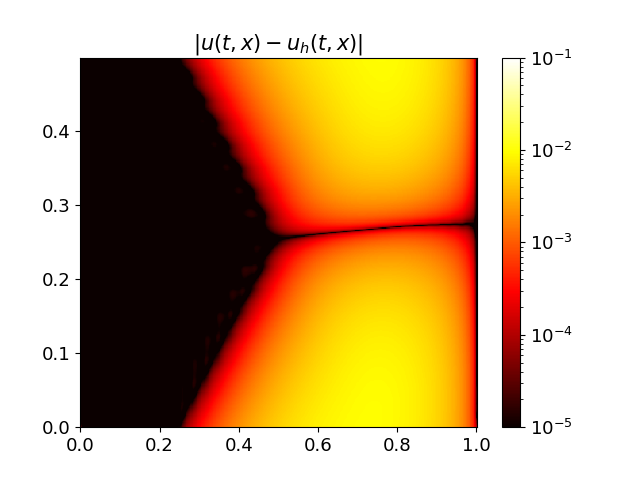
\includegraphics[scale = 0.3 ]{abs-err.png}};
\draw[->,ultra thick] (-2.35,-0.95) -- node [right,at end] {$x$}  (1.0,-0.95);
\draw[->,ultra thick] (-2.35,-0.95) -- node [above,at end] {$t$}  (-2.35,2.5);
\draw[white,ultra thick,dashed] (-1.05,-0.5 ) -- (-0.3, 1.0);
\draw[white,ultra thick,dashed] (-0.3,1.0 ) -- (-1.05, 2.4);
\node[] (B) at (-1.3,0.95) {  $\textcolor{white}{B}$ };
\draw[lightgray,ultra thick, ->] (-2.0,1.15 ) -- (-4.8, 0.95);
 \end{scope}


\begin{scope}[xshift=8.65cm]
\begin{tiny}
\begin{axis}[ 
    height = 4.15cm,
    width = 5.45cm,
    name=vel,
    ymode=log,
    xmode=log,
    ymax = 1e-0,
    axis y line*=left,
    xlabel= { $\Delta t = h$},
    ytick = {1e-3,1e-5},
    legend style = { column sep = 10pt, legend columns = 1, legend to name = grouplegendnoGCCv,},
    x label style={at={(axis description cs:0.75,+0.31)},anchor=east},
    y tick label style={ xshift=2.85em,yshift=-0.4em },
    %title = { $\norm{ \partial_t(\cdot) }_{L^{2}(0,T;L^2(\Omega))}$  vs. $\norm{ \partial_t(\cdot) }_{L^{2}(0,T;L^2(B_t))}$ },
    %title = { $L^{2}(0,T;L^2(\Omega))$  vs. $\norm{ \partial_t(\cdot) }_{L^{2}(0,T;L^2(B_t))}$ },
    title = { $\partial_t u$ in $ \Omega$ (solid) vs $ B_t $ (dashed) },
    title style={at={(0.5,1.0735)},anchor=north},
    legend style={at={(0.5,-0.1)},anchor=north},
	]
    \addplot[red,very thick,mark=*,forget plot]
        table[x=deltat,y=L2L2ut-all] {../data/noGCC-restricted-1d-order1.dat}; \addlegendentry{$q=k=1$}%
    \addplot[blue,very thick,mark=triangle,forget plot] 
        table[x=deltat,y=L2L2ut-all] {../data/noGCC-restricted-1d-order2.dat};  \addlegendentry{$q=k=2$}%
    \addplot[green!70!black,very thick,mark=x,forget plot]
        table[x=deltat,y=L2L2ut-all] {../data/noGCC-restricted-1d-order3.dat};  \addlegendentry{$q=k=3$}%

    \addplot[red,very thick,mark=*,dashed,forget plot]
        table[x=deltat,y=L2L2ut-restrict] {../data/noGCC-restricted-1d-order1.dat};  %\addlegendentry{$q=k=1$}%
    \addplot[blue,very thick,mark=triangle,dashed,forget plot]
        table[x=deltat,y=L2L2ut-restrict] {../data/noGCC-restricted-1d-order2.dat}; %\addlegendentry{$q=k=2$}%
    \addplot[green!70!black,very thick,mark=x,dashed,forget plot]
        table[x=deltat,y=L2L2ut-restrict] {../data/noGCC-restricted-1d-order3.dat};  %\addlegendentry{$q=k=3$}%

    \addplot[lightgray,dashed,ultra thick]
        table[mark=none,x=deltat,y expr ={1.3*\thisrowno{0}}] {../data/noGCC-restricted-1d-order1.dat};  \addlegendentry{$ \mathcal{O}(\Delta t) $ } %
    \addplot[lightgray,dotted,ultra thick]
        table[mark=none,x=deltat,y expr ={0.4*\thisrowno{0}*\thisrowno{0} }] {../data/noGCC-restricted-1d-order2.dat};  \addlegendentry{$ \mathcal{O}((\Delta t)^2) $ } %
    \addplot[lightgray,dashdotted,ultra thick]
        table[mark=none,x=deltat,y expr ={.1*\thisrowno{0}*\thisrowno{0}*\thisrowno{0}}] {../data/noGCC-restricted-1d-order3.dat};  \addlegendentry{$ \mathcal{O}((\Delta t)^3) $ } %     
    %\legend{ $q=k=1$, $q=k=2$,$q=k=3$ } 
    %\node[draw,circle,ultra thick,lightgray] (Z1) at (axis cs:0.0625,6.5e-3) {};
   \end{axis}
    \node at ($(vel) + (-0.0cm,-2.25cm)$) {\ref{grouplegendnoGCCv}}; 
\end{tiny}
\end{scope}
\end{tikzpicture}
\end{center}
\label{fig:NoGCC-1D-B}
\end{figure}

\end{document}

